\label{chap:inverse_model}

\begin{figure}[ht]
	\centering
	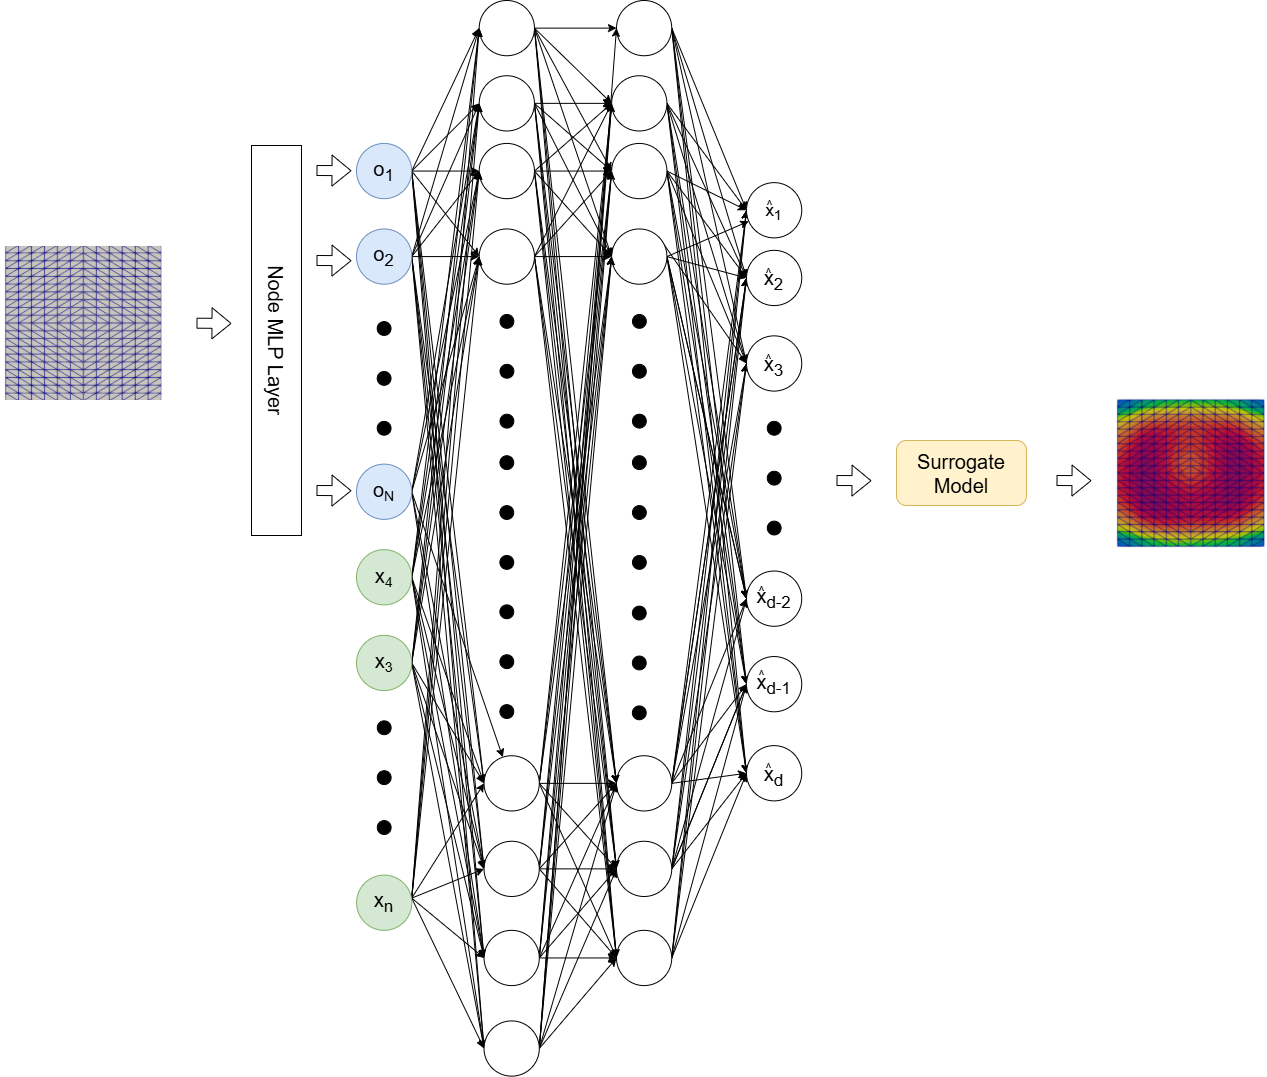
\includegraphics[width=0.6\linewidth]{figures/mesh_mlp.png}
	\caption{Inverse model architecture}
	\label{fig:inverse_model}
\end{figure}


The objective of the inverse model $\mathcal{I}$ is, given a target temperature distribution at the core of the sheet, to infer the machine parameter configuration capable of reproducing it.

In contrast to the surrogate model $\mathcal{S}$, $\mathcal{I}$ does not employ an MGNN architecture, as it is required to output continuous-valued machine parameters that are not inherently associated with mesh nodes, which instead serve as input features.

To preserve the positional temperature information associated with the mesh, the architecture of $\mathcal{I}$ processes node-level information through a Node MLP layer, as illustrated in Figure~\ref{fig:node_mlp}, followed by a fully connected network, as shown in Figure~\ref{fig:inverse_model}.

The input size of the Node MLP layer remains fixed across the dataset. All instances share the same number of mesh nodes, while the mesh is geometrically stretched or compressed according to the sheet geometry of each example.

\begin{figure}[t]
	\centering
	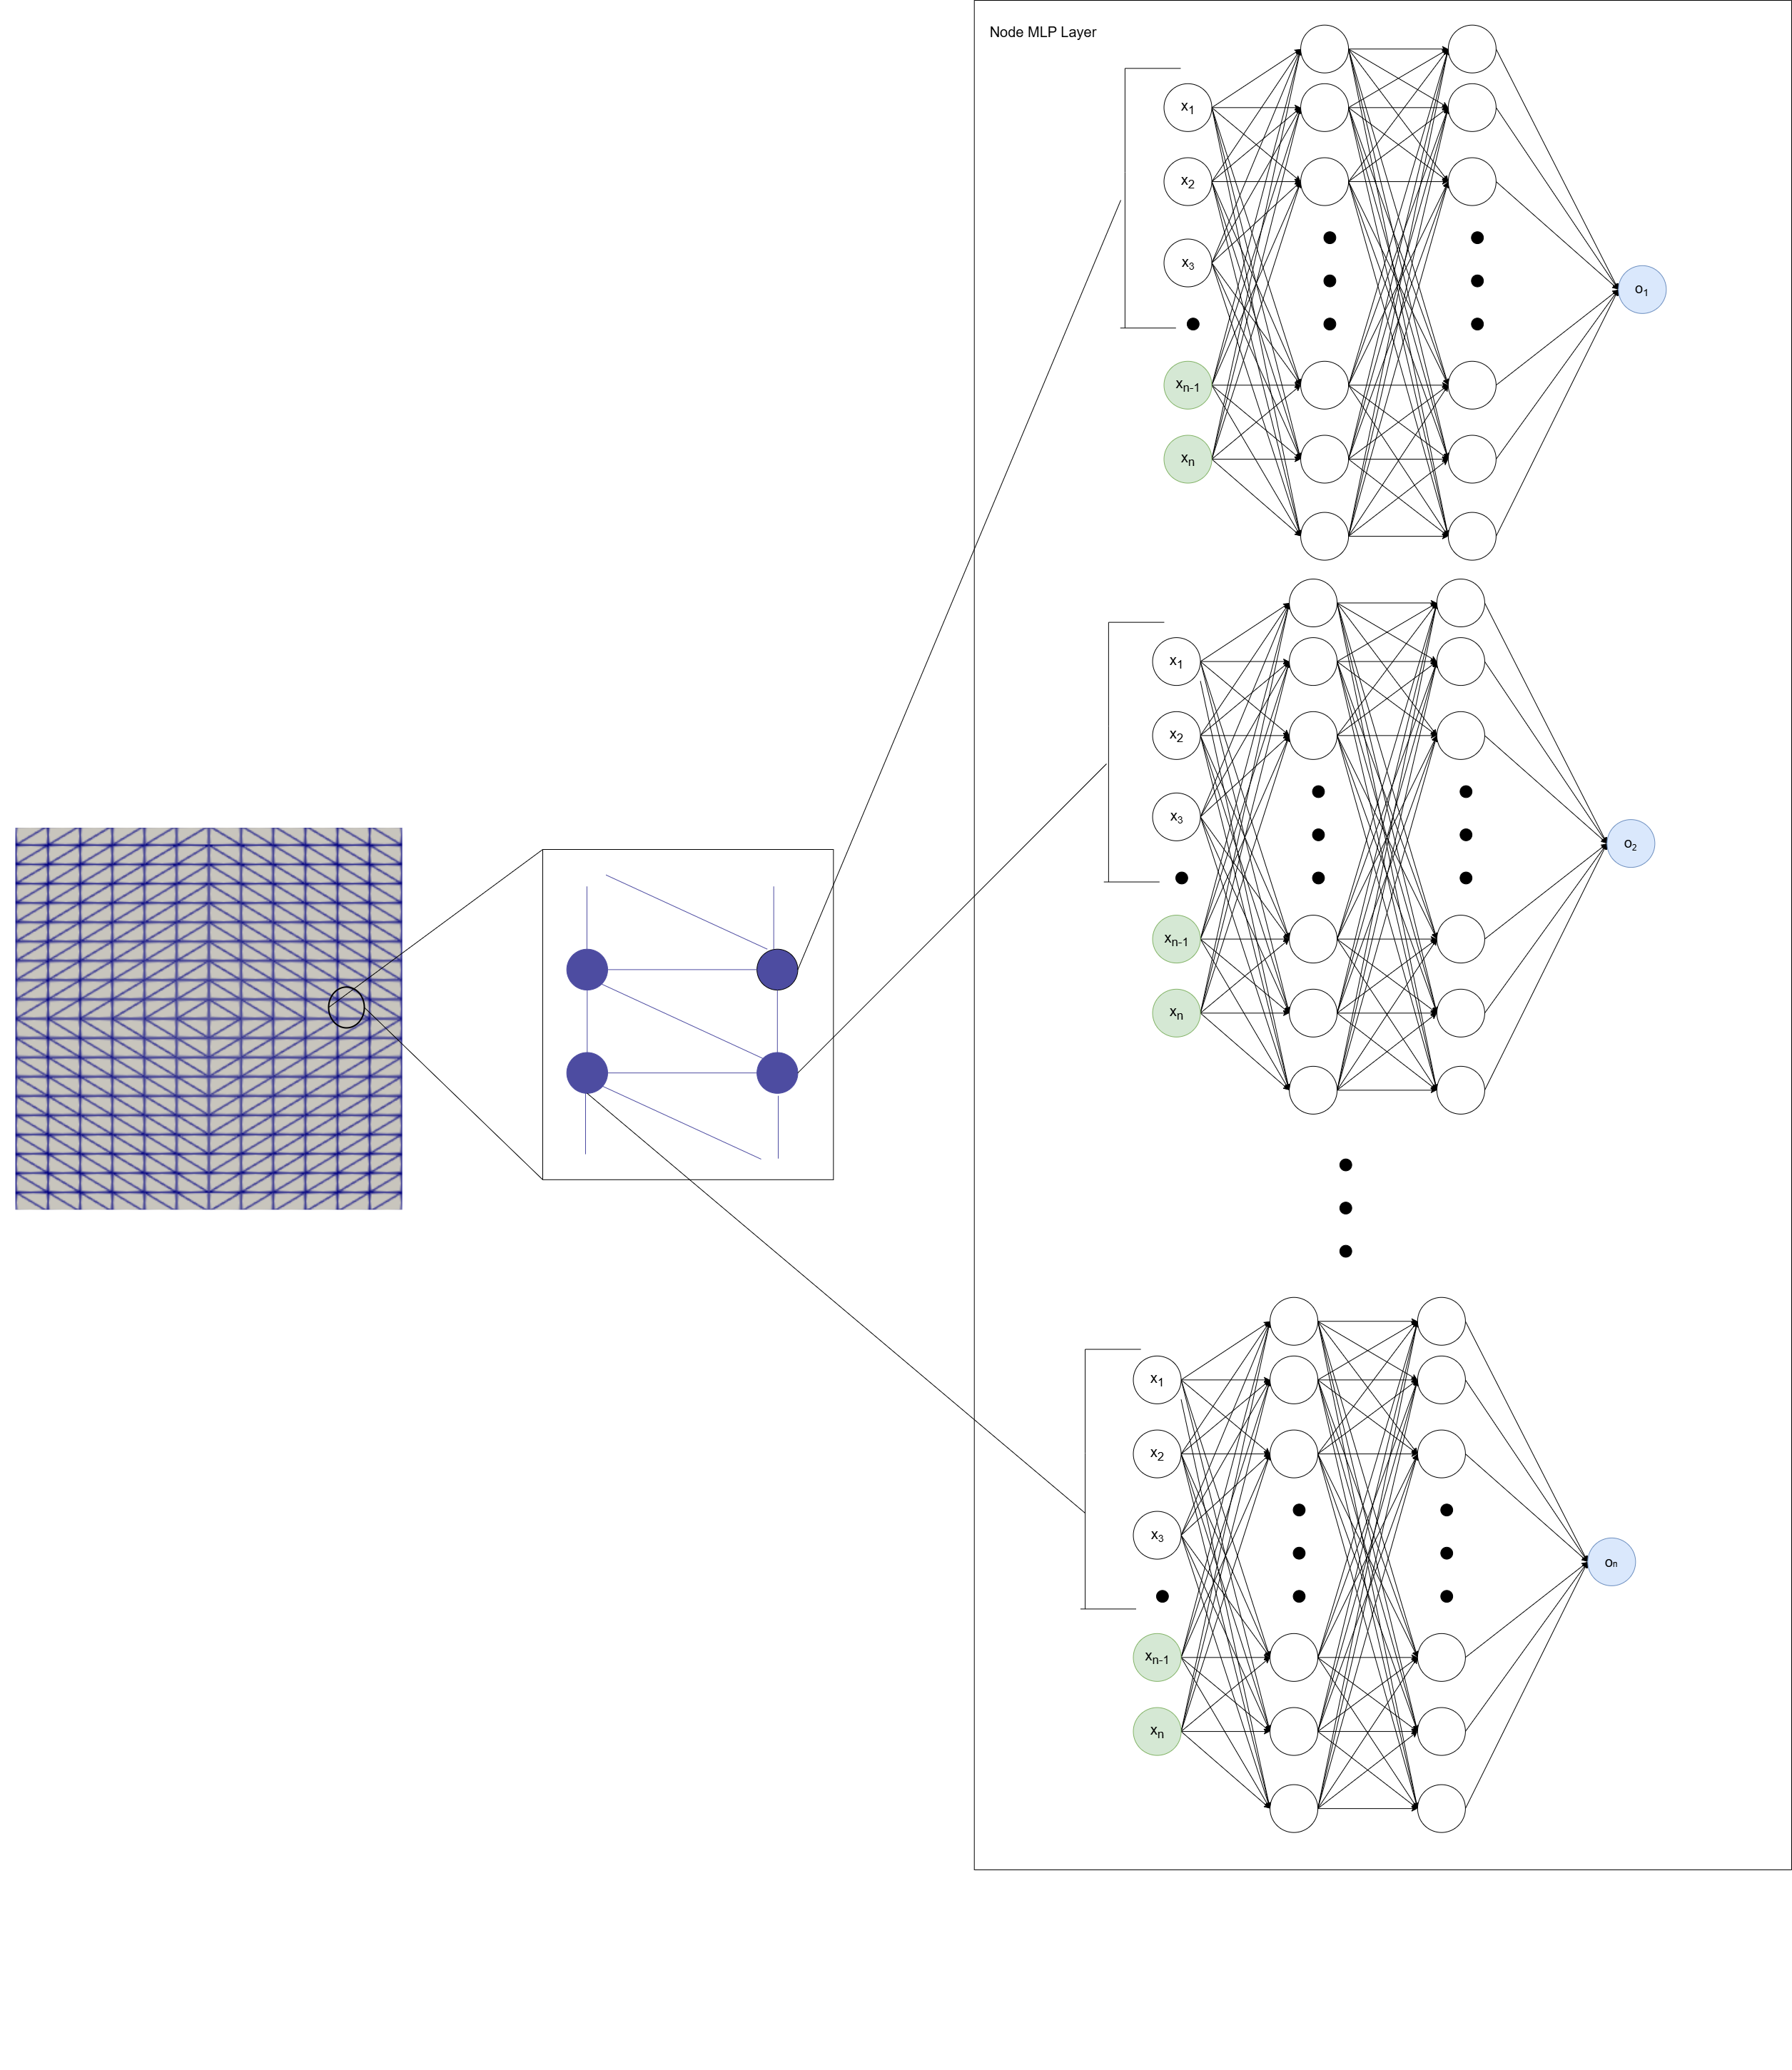
\includegraphics[width=0.5\linewidth]{figures/node_mlp_layer.png}
	\caption{Node MLP layer}
	\label{fig:node_mlp}
\end{figure}

The Node MLP layer consists of a distinct MLP for each mesh node, each composed of two fully connected hidden layers with 16 units. The input to each node-specific MLP includes the mesh node coordinates, the desired temperature at the corresponding node, the sheet geometry (width, height, thickness), and the material properties (volumetric heat capacity, surface emissivity, and thermal conductivity). The sheet characteristics are repeated for each node, as this redundancy has been observed to yield better performance during training than excluding this information.

Each node MLP produces a single output $\mathbf{o}_i$, representing the processed information for node $i$ of the mesh. These outputs are then concatenated with the geometric and material properties of the sheet and processed by a subsequent fully connected network consisting of two hidden layers with 512 units each.

The inverse model predicts a 245-dimensional vector corresponding to the input required by $\mathcal{S}$, excluding the sheet geometry, and material properties, which are shared inputs between both models.

A key component of the output concerns the lamp powers configuration. In the real industrial scenario, machine operators always deactivate lamps outside the sheet area, while setting boundary lamps to the maximum capacity. This prior knowledge is embedded into the model through a masking mechanism applied during training, which prevents updates to the weight corresponding to the already known lamps values, improving convergence stability.

The model is trained using the loss function $\mathcal{L}_i$ expressed in Eq.~\ref{eq:loss_inverse} and optimized using Adam with a learning rate of $1 \times 10^{-2}$. Training is performed with a batch size of 64 for up to 1000 epochs, with early stopping selecting the final model at epoch 842. The training is conducted on the same hardware setup used for the surrogate model and requires approximately four days.

\section{Loss function formulation}
\label{sec:inverse_loss_function}

The inverse problem is inherently ill-posed, since multiple machine configurations may produce similar temperature distributions. Therefore, the objective is not exact reconstruction of simulator inputs, but rather the identification of physically consistent and cost-efficient solutions.

The inverse model prediction $\mathbf{\hat{x}}$ is evaluated through the surrogate model as $\mathbf{\hat{y}} = \mathcal{S}(\mathbf{\hat{x}})$. From the obtained output $\mathbf{\hat{y}}$, we extract the predicted core temperature distribution $\mathbf{\hat{y}}_C$, the maximum temperatures at the top and bottom of the sheet $(\mathbf{\hat{y}}_T, \mathbf{\hat{y}}_B)$, the net heating time $\mathbf{\hat{y}}_H$, and the energy consumption $\mathbf{\hat{y}}_E$.

The temperature error is defined as:
\begin{equation}
	E_T = \frac{1}{n} \sum_{i=1}^{n} \left( \mathbf{\hat{y}}_{C,i} - \left(\mathbf{y}_{C,i} + \frac{\epsilon}{2}\right) \right)^2
\end{equation}

\noindent where $\epsilon = 3~^\circ\mathrm{C}$ defines a temperature tolerance. Shifting the target by $\epsilon/2$ introduces a safety margin that encourages the model to avoid under-heating, which was observed during preliminary experiments.

Process cost is computed as:
\begin{equation}
	P_{\mathrm{Cost}} = \frac{1}{n} \sum_{i=1}^{n} \left( \frac{h}{3600} \mathbf{\hat{y}}_{H,i} + e \mathbf{\hat{y}}_{E,i} \right)
	\label{eq:cost}
\end{equation}

\noindent where $h$ and $e$ are machine-hour cost and energy cost coefficients, respectively.

To ensure material safety constraints, we introduce a penalty term for configurations in which the top surface maximum temperature exceeds the maximum core temperature by more than $\gamma = 15~^\circ\mathrm{C}$:
\begin{equation} 
	\lambda = \frac{1}{n} \sum_{i=1}^{n} \max\left( (\mathbf{\hat{y}}_{T,i} - \mathbf{\hat{y}}^{\max}_{C,i} - \gamma)^2, 0 \right)
	\label{eq:penalty} 
\end{equation}

Only the top surface temperature is considered in this penalty term, as preventing overheating on the top surface, which corresponds to the visible side of the final product, is of primary importance. In contrast, the bottom surface is in contact with the mould during forming and is therefore less critical in terms of thermal degradation.

As for the surrogate model, a sigmoid weighting term balances temperature distribution accuracy and cost minimization:
\begin{equation}
	\sigma = \text{sigmoid} \left( \frac{E_T - \epsilon^2}{\tau \cdot \epsilon^2} \right)
\end{equation}

The final loss is defined as:
\begin{equation}
	\mathcal{L}_i = \sigma E_T + (1 - \sigma) P_{\mathrm{Cost}} + \lambda
	\label{eq:loss_inverse}
\end{equation}

This formulation ensures that the model prioritizes temperature accuracy when errors are significant and progressively shifts its focus toward cost efficiency once thermal targets are sufficiently satisfied, while maintaining safety constraints throughout training.

\section{Model assessment}

\begin{figure}[h]
	\centering
	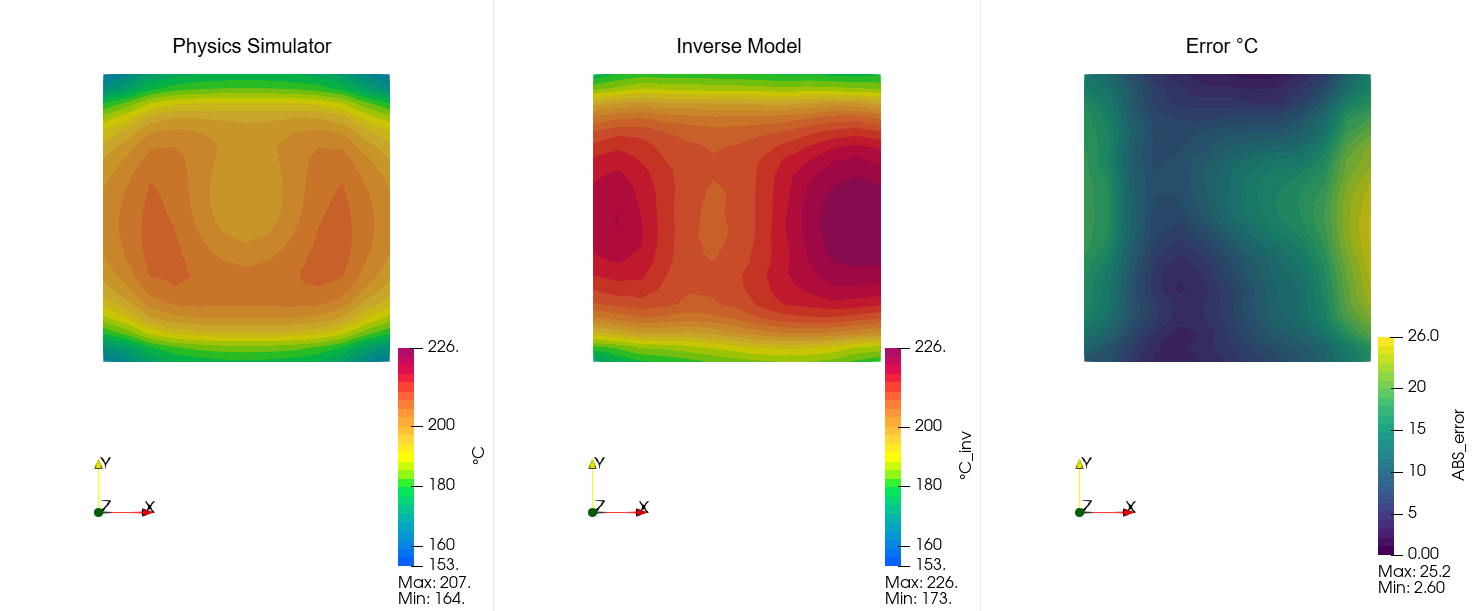
\includegraphics[width=0.7\linewidth]{figures/inverse_model_with_label.png}
	\caption{Prediction example on the test set. From left to right: the temperature distribution obtained from the physics-based simulator, the prediction produced by the inverse model, and the absolute error between the target temperature distribution and the predicted one.}
	\label{fig:inverse_model_prediction}
\end{figure}

At the end of training, evaluation of the temperature distribution revealed a maximum average absolute error of 15.33$^\circ\mathrm{C}$ on the training set, 15.36$^\circ\mathrm{C}$ on the validation set and 22.99$^\circ\mathrm{C}$ on the test set.

Figure~\ref{fig:inverse_model_prediction} illustrates the same test case shown in Figure~\ref{fig:surrogate_model_prediction}, using the inverse model prediction. The model successfully captures the spatial heating strategy, increasing temperatures along the lateral regions while maintaining lower values in the central region and along the top and bottom edges of the sheet.

The error is mainly concentrated on the right-hand side of the sheet, while remaining low in the central and boundary regions. This temperature deviation arises from the inverse model’s tendency to favor higher lamp power configurations, reflecting the learned trade-off between energy usage and processing time, where shorter high-power heating cycles are more cost-efficient than prolonged low-power operation.

Quantitatively, the inverse model achieves an average cost reduction of 49.53\% on the training set, of 49.40\% on the validation set and of 34.52\% on the test set.

Although the results are satisfactory, since the model is trained on simulator-generated data, reducing the temperature deviation with respect to the target distribution is important to improve robustness when applied to real industrial scenarios, where sheet characteristics and operating conditions may vary across cases. 

For this reason, a targeted optimization step is applied at the individual-instance level, starting from the inverse model output. This step primarily reduces the temperature distribution error and subsequently refines the process cost, balancing the trade-off between thermal accuracy and cost minimization.